%-*-coding:UTF-8-*-
%《地球物理反演理论与方法》结课作业
\documentclass[hyperref,UTF-8,twoside]{ctexart}
\newcommand*\bigglabs[1]{\biggl\lvert#1\biggl\rvert}
\newcommand*\abs[1]{\lvert#1\rvert}
\newcommand{\cndash}{\rule{0.2em}{0pt}\rule[0.35em]{1.6em}{0.05em}\rule{0.2em}{0pt}}
\hypersetup{colorlinks=false,pdfborder=000}
\usepackage{geometry}
\usepackage{amsmath}
\usepackage{makecell}
\renewcommand{\rmdefault}{ptm}
\geometry{a4paper,centering,scale=0.8}
\title{\heiti《地球物理反演理论与方法》结课作业}
\usepackage{txfonts}
\usepackage{upgreek}
\usepackage{multirow,makecell}
\usepackage{fancyvrb}
\usepackage{pifont}
\numberwithin{equation}{section}
\begin{document}
\zihao{4}
\begin{titlepage}
\vspace*{40mm}
\begin{center}
{\heiti\Huge《地球物理反演理论与方法》结课作业}\\[5mm]
{\heiti\huge \cndash{}电阻率测深一维反演}\\[30mm]
{\Large 王亮}\\[5mm]
地质资源与地质工程\\\texttt{学号:102014079}\\[80mm]
2015年7月1日
\end{center}
\end{titlepage} 
\thispagestyle{empty}
\mbox{} 
\newpage
\thispagestyle{empty}
\pagenumbering{roman}
\tableofcontents
\newpage
\thispagestyle{empty}
\mbox{} 
\newpage
\begin{abstract}
\pagenumbering{arabic}
这是我的《地球物理反演理论与方法》课程的结课作业。在这份结课作业中,我编写了直流电测深一维正反演程序。
\end{abstract}
\section{电阻率测深法原理}
通常,电阻率法是通过观测地表的电场来了解地下介质电性分布的。
这就要求目标地层的存在对观测点处的电场有明显的扰动。
因为在电阻率法中都是使用点电流源,因此需要考察距离点电流源不同距离时透入某一给定深度以下供电电流所占比例的变化规律。
在相距$2L$的两个异性点电流源$AB$之间的中垂面上任意一点上的电流密度为:
\begin{equation}
J = \frac {IL } {\uppi} \frac{1}{(L^2+y^2+z^2)^{\frac{3}{2}}}
\end{equation}
式中,$y$为观测点距$AB$连线的水平距离;$z$为深度;$I$为供电电流强度。透入给定深度z以下的相对电流强度为:
\begin{equation}
\frac{I_z}{I}=\frac{L}{\uppi}\int_{-\infty}^{\infty}\int_{z}^{\infty} \frac{dydz}{(L^2+y^2+z^2)^{\frac{3}{2}}}
\end{equation}

在研究地下介质电阻率的垂向变化时,希望尽量减小横向电阻率变化的影响。
如前所述,移动测量电极$MN$对地下介质电阻率的横向变化反映非常明显,而移动供电电极$AB$对地下介质电阻率的横向变化反映则远没有那么明显。
为了减少横向电阻率变化的影响,应该采用一种测量电极$MN$基本保持不动,主要移动供电电极$AB$的装置。
在实际工作中,一般采用对称四极测深装置,在施工条件限制时,也可采用三极测深装置,其他装置则很少使用。
\section{多层水平地层上视电阻率表达式}
\subsection{水平地层上地面点电流源的电场}
假定地面水平,在地下有n层水平层状地层,各层的电阻率分别为$\rho_1,\rho_2,\ldots,\rho_n$;
厚度分别为$h_1,h_2,\ldots,h_n$,其中$h_n\to\infty$;每层地面到地面的距离为$H_1,H_2,\ldots,H_n$,其中$H_n\to\infty$。
在$A$点有一电流源供电,电流强度为$I$。

用柱坐标系,将原点设在$A$点,$z$轴垂直向下。由于问题的解具有轴对称性,与$\psi$无关,因此电位分布满足以下形式的拉普拉斯方程:
\begin{equation}
\frac {\partial^2U} {\partial{r^2}} +\frac{1}{r}\frac{\partial{U}} {\partial{r}}+\frac {\partial^2U} {\partial{z^2}}=0\label{eq:3-1}
\end{equation}
以及如下边界条件:
\begin{enumerate}
\item 电源点附近,趋于地面点电流源的正常电位,即
\begin{equation}
\lim_{R=sqrt{r^2+z^2}\to0}U_1=\frac{I\rho_1}{2\uppi{R}}\label{eq:3-2}
\end{equation}
\item 在地面处电流密度法向分量为零,即
\begin{equation}
\frac{1}{\rho_1}\frac{\partial{U_1}}{\partial{z}}\Bigg\vert_{z=0}=0\label{eq:3-3}
\end{equation}
\item 除场源点外,电位处处有限,且无穷远处电位为零,即
\begin{equation}
U_{{n_z}\to\infty}\to0
\end{equation}
\item 在岩层分界面处电位连续,即
\begin{equation}
U_{i_{z=H_i}}=U_{{i+1}_{z=H_i}}\label{eq:3-4}
\end{equation}
其中,$i=1,2,\ldots,n-1$.
\item 在岩层分界面处电流密度法向分量连续,即
\begin{equation}
\frac{1}{\rho_i}\frac{\partial{U_i}}{\partial z}_{z=H_i}=\frac{1}{\rho_{i+1}}\frac{\partial{U_{i+1}}}{\partial z}_{z=H_i}\label{eq:3-5}
\end{equation}
其中$i=1,2,\ldots,n-1$。
\end{enumerate}
式(\ref{eq:3-1})可用分离变量法求解,设
\begin{equation}
U=R(r)Z(z)\label{eq:3-6}
\end{equation}
经分离变量后得到两个二阶常微分方程
\begin{equation}
\frac{\partial^2{R}}{\partial{r^2}}+\frac{1}{r}\frac{\partial{R}}{\partial r}+m^2R=0\label{eq:3-7}
\end{equation}
\begin{equation}
\frac{\partial^2{Z}}{\partial{z^2}}-m^2Z=0\label{eq:3-8}
\end{equation}
其中,式(\ref{eq:3-7})的解为第一类和第二类零阶贝塞尔函数和。第二类零阶贝塞尔函数在$r=0$的$Z$轴上趋于无穷,这种特征不符合点场源特征,因此应舍去,这样式(\ref{eq:3-7})的解为第一类零阶贝塞尔函数。式(\ref{eq:3-8})的解为
\begin{equation}
Z(z)=Ae^{-mz}+Be^{mz}\label{eq:3-9}
\end{equation}
由此可写出各层电位积分形式的通解
\begin{equation}
U_{i}(r,z)=\frac{I}{2\uppi}\int_0^\infty[A_i(m)e^{-mz}+B_i(m)e^{mz}]J_0(mr)dm\label{eq:3-10}
\end{equation}
式中,$ A_i(m)$和$B_i(m)$为待定函数; $i=1,2,\ldots,n$。
在第一层介质中的电位,还应附加电源点电位,即
\begin{equation}
U_{1}(r,z)=\frac{I\rho_1}{2\uppi{R}}+\frac{I}{2\uppi}\int_0^\infty[A_i(m)e^{-mz}+B_i(m)e^{mz}]J_0(mr)dm\label{eq:3-11}
\end{equation}
由
\begin{equation}
\frac{\partial U_1(r,z)}{\partial z}=\frac{I\rho_{1}z}{2\uppi(r^2+z^2)^\frac{3}{2}}+\frac{I}{2\uppi}\int_0^\infty[-A_1(m)e^{-mz}+B_1(m)e^{mz}]mJ_0(mr)dm
\end{equation}
据边界条件式(\ref{eq:3-3}),可得
\begin{equation}
A_1(m)=B_1(m)
\end{equation}
又根据李普希积分:
\begin{equation}
\frac{1}{R}=\int_0^\infty e^{-m\abs{z}}J_0(mr)dm\label{eq:3-12}
\end{equation}
得
\begin{equation}
U_1(r,z)=\frac{1}{2\uppi}\int_0^\infty\{[\rho_1+B_1(m)]e^{-mz}+B_1(m)e^{mz}\}J_0(mr)dm\label{eq:3-13}
\end{equation}
在第n层介质中么,当时,电位有限,因此,
\begin{equation}
U_n(r,z)=\frac{1}{2\uppi}\int_0^\infty A_n(m)e^{-mz}J_0(mr)dm\label{eq:3-14}
\end{equation}
代入边界条件后可得到地面电位的表达式
\begin{equation}
U_1(r)=\frac{1}{2\uppi}\int_0^\infty T_1(m)J_0(mr)dm\label{eq:3-15}
\end{equation}
式中,为电阻率转换函数。注意到,可得到的递推公式为 
\begin{equation}
T_n=\rho_n
\end{equation}
\begin{equation}
T_i=\rho_i{\frac{(T_{i+1}+\rho_i)+(T_{i+1}-\rho_i)e^{-2mh_i}}{(T_{i+1}+\rho_i)-(T_{i+1}-\rho_i)e^{-2mh_i}}}\label{eq:3-16}
\end{equation}
\subsection{水平地层上视电阻率表达式及滤波算法}
式(\ref{eq:3-15})对$r$微分,得电场强度
\begin{equation}
E_r=-\frac{\partial{U_1(r)}}{r}=\frac{I}{2\uppi}\int_0^\infty{T_1(m)mJ_1(mr)dm}\label{eq:3-17}
\end{equation}
由此得到时的对称四极装置视电阻率表达式
\begin{equation}
\rho_s=r^2\int_0^\infty{T_1(m)mJ_1(mr)dm}\label{eq:3-18}
\end{equation}
其中$r$是供电极距$\frac{AB}{2}$

在电测深视电阻率的表达式中的被积函数可以分为两部分,一是包含地下各层所有信息(厚度及电阻率)的电阻率转换函数,二是与地层参数无关的贝塞尔函数,虽然没有解析计算结果,但可用线性滤波方法进行计算。根据电阻率转换函数的变化规律,对的抽样取对数等间隔比较合适,因此,首先令,则电阻率的表达式变为
\begin{equation}
\rho_{s}(r)=\int_{-\infty}^\infty{T_1(\frac{e^x}{r})e^{2x}J_1(e^x)dx}\label{eq:3-19}
\end{equation}
根据采样定理,一个函数可以用它在等间距离散抽样点上的抽样值表达
\begin{equation}
f(x)=\sum_{k=-\infty}^{\infty}f(k\Delta x)\frac{sin[\frac{\uppi(x-k\Delta x)}{\Delta x}]}{\frac{\uppi(x-k\Delta x)}{\Delta x}}\label{eq:3-20}
\end{equation}
将电阻率装换函数用它在数轴上的离散抽样值表达为
\begin{equation}
T_1(\frac{e^x}{r})=\sum_{k=-\infty}^{\infty}T_1(\frac{e^{k\Delta x}}{r})\frac{sin[\frac{\uppi(x-k\Delta x)}{\Delta x}]}{\frac{\uppi(x-k\Delta x)}{\Delta x}}\label{eq:3-21}
\end{equation}
记
\begin{equation}
C_k=\int_{-\infty}^{\infty}\frac{sin[\frac{\uppi(x-k\Delta x)}{\Delta x}]}{\frac{\uppi(x-k\Delta x)}{\Delta x}}e^{2x}J_1(e^x)dx\label{eq:3-22}
\end{equation}
则
\begin{equation}
\rho_s(r)=\sum_{k\to -\infty}^{\infty}T_1(\frac{e^{k\Delta x}}{r})C_k\label{eq:3-23}
\end{equation}
将$C_k$预先计算出来,实际上取有限项求和就可以达到足够的精度了。
从频谱分析的观点看,当电阻率装换函数用它在数轴上的离散抽样值表达式时,相当于滤取了频率高于的谐波成分,因此这种计算视电阻率的方法称为滤波计算方法,称为滤波系数。
为了提高线性滤波计算的精度,减少滤波系数的数目,需要对的抽样点进行位移,实际使用的线性滤波计算视电阻率的公式为
\begin{equation}
\rho_s(r)=\sum_{k=k_1}^{k_2}T_1(\frac{e^{k\Delta x+s}}{r})C_k\label{eq:3-24}
\end{equation}
式中,$\rho_s(r)$为供电极距为$r$时的视电阻率;$T_1(\frac{e^{k\Delta x+s}}{r})$为$m=\frac{e^{k\Delta x+s}}{r}$时的电阻率转换函数;$C_k$为第$k$个滤波系数;$\Delta x$为抽样间隔;$s$为位移系数。

实际线性滤波计算常用的抽样间隔有两种。一种为六点是抽样间隔,即$\Delta x=\frac{ln10}{6}=10^\frac{1}{6}$,直流电阻率测深曲线一般都采用这种抽样间隔进行计算。另一种为十点式抽样间隔,即$\Delta x=\frac{ln10}{10}=10^\frac{1}{10}$,电磁测深曲线一般都采用这种抽样间隔进行计算。

下表为常用的一套六点式抽样间隔的滤波系数,共有20个系数:$k=1,\ldots,20$,其位移系数$s=-2.1719$,$e^-2.1719=0.11396$。
用上述公式就可计算某个供电极距$r$的视电阻率,只要计算20个对应于这个供电极距的不同值的电阻率转换函数$T_1(m_k)$,将其与下表中对应的20个滤波系数相乘再求和就可以了。
\begin{center}
\renewcommand\arraystretch{1}
\begin{tabular}{|c|c|c|c|c|c|c|c|}
\Xhline{1.5pt}
$K$&1&2&3&4&5&6&7\\\hline
$C(k)$&0.003042&-0.001198&0.01284&0.0235&0.08688&0.2374&0.6194\\
\Xhline{1.5pt}
$K$&8&9&10&11&12&13&14\\\hline
$C(k)$&1.1817&0.4248&-3.4507&2.7044&-1.1324&0.393&-0.1436\\
\Xhline{1.5pt}
$K$&15&16&17&18&19&20&\\\hline
$C(k)$&0.05812&-0.02521&0.01125&-0.004978&0.002072&-0.000318&\\
\Xhline{1.5pt}
\end{tabular}
\end{center}
\vspace{15pt}

因为要计算一条视电阻率测深曲线就需要计算多个供电极距的视电阻率,为减少计算量,取$r_i=e^{i\Delta x}=10^{\frac{1}{6}}$,则$m_k=e^{\frac{k\Delta x+s}{r_i}}=e^{(k-i)\Delta x+s}=0.11396*10^{\frac{k-i}{6}}$,这样,计算不同供电极距的视电阻率所需要的电阻率转换函数大多数可以共用。
这样取值时,线性滤波计算视电阻率的公式可以写为
\begin{equation}
\rho_s(r_i)=\sum_{k=1}^{20}T_1(m_{k-i})C_k\label{eq:3-25}
\end{equation}
下面是用数值滤波法计算视电阻率测深曲线的计算机流程:
\begin{enumerate}
\item 输入层参数,包括层数$n$、各层的层厚度$h_i$和电阻率$\rho_i$;
\item 输入要计算的供电极距范围,并由此得到$r=e^{i\Delta x}$中$i$的变化范围:$(i_{min},i_{max})$;
\item 计算$k-i$的变化范围:$((k-i)_{min},(k-i)_{max})$;
\item 用电阻率转换函数递推公式,循环计算$m_j=e^{j\Delta x+s}=0.11396*10^{\frac{j}{6}}$,$j=(k-i)_{min},\ldots,(k-i)_{max}$时的;
\item 用滤波公式循环计算$r_i=e^{i\Delta},i=i_{min},\ldots,i_{max}$时的$\rho_s(r_i)$。
\end{enumerate}
\section{自动反演法理论}
反演是由响应到模型的过程,是正演的逆过程,对水平层状大地对称四极电阻率测深曲线的解释就是反演问题,主要解释方法有四种:特征点法、直接反演法、正演拟合法,自动反演法。
由于计算机的便利,我们通常采用自动反演法。

电阻率测深数据的自动反演方法可归结为寻找模型$M(M_j,j=1,2,\ldots,NM)$使下面的目标函数$\varphi$趋于极小:
\begin{equation}
\varphi=\sum_{i=1}^{NS}\bigglabs{\rho_{si}-\rho_{ai}(M)}^\alpha\label{eq:4-1}
\end{equation}
式中, $\rho_{si}$是第$i$个极距的实测视电阻率,$M(M_j,j=1,2,\ldots,NM)$是由模型$M$正演计算所得的第$i$个极距的理论视电阻率,$M_j,j=1,2,\ldots,NM$是模型参数(地层的电阻率或厚度),$NM$是模型参数个数,$NS$是供电极距数,$\alpha$是范数,当$\alpha=2$时即为最小二乘法。将模型$M$在预测模型处展开,并忽略二次项以上的项,式(\ref{eq:4-1})表达可改为求预测模型修改量$\Delta M$使目标函数$\varphi$趋于极小:
\begin{equation}
\varphi=\sum_{i=1}^{NS}\bigglabs{\rho_{si}-\rho_{ai}-\sum_{j=1}^{NM}\frac{\partial \rho_{ai}}{\partial M_j}\Delta M_j}^\alpha\label{eq:4-2}
\end{equation}
式(\ref{eq:4-2})要趋于极小,则对于各供电极距$i(i=1,2,\ldots,NS)$要满足下面的线性方程:
\begin{equation}
\sum_{j=1}^{NM}\frac{\partial \rho_{ai}}{\partial M_{j}}\Delta M_j=\rho_{si}-\rho_{ai}\label{eq:4-3}
\end{equation}
解上述线性方程组,就可得到预测模型$M$的修改量$\Delta M$,于是可得到新的预测模型,计算新模型的理论视电阻率,与实测视电阻率进行对比,如果精度满足要求,则新的预测模型即为反演结果;否则重新展开,计算模型修改量,直到满足要求。

下面是对反演过程的三个具体问题的具体处理方法。
\begin{enumerate}
\item 偏导数的计算
\begin{itemize}
\item 可用差分方法来计算,取$\Delta M_j=0.1M_j$,则
\begin{equation}
\frac{\partial \rho_{ai}}{\partial M_j}=\frac{\rho_{ai}(M_1,M_2,\ldots,1.1M_j,\ldots,M_{NM})-\rho_{ai}(M_1,M_2,\ldots,M_j,\ldots,M_{NM})}{0.1M_j}\label{eq:4-4}
\end{equation}
\end{itemize}
\item 模型参数的处理
\begin{itemize}
\item 模型参数中有不同量纲的电阻率和厚度,尤其对电阻率参数,变化范围很大,如果直接由上述方法求解,不但会导致方程(\ref{eq:4-3})严重病态,而且电阻率和厚度参数的修改量也不会正确,从而导致反演方法不收敛。
为了解决这个问题,可对方程(\ref{eq:4-3})无量纲化。
将式(\ref{eq:4-4})的偏导数代入方程式(\ref{eq:4-3})中,有
\begin{equation}   \begin{split}
&\sum_{j=1}^{NM}10[\rho_{ai}(M_1,M_2,\ldots,1.1M_j,\ldots,M_{NM})-\\
&\rho_{ai}(M_1,M_2,\ldots,M_j,\ldots,M_{NM})]\frac{\Delta M_j}{M_j}\\
&=\rho_{si}-\rho_{ai}(M_1,M_2,\ldots,M_j,\ldots,M_{NM})\label{eq:4-5}
\end{split}    \end{equation}
其中,$i=1,2,\ldots,NS$
上式两端同时除以$\rho_{ai}(M_1,M_2,\ldots,M_j,\ldots,M_{NM})$得
\begin{equation}
\sum_{j=1}^{NM}10[\frac{\rho_{ai}(M_1,M_2,\ldots,1.1M_j,\ldots,M_{NM})}{\rho_{ai}(M_1,M_2,\ldots,M_j,\ldots,M_{NM})}-1]\frac{\Delta M_j}{M_j}=\frac{\rho_{si}}{\rho_{ai}}-1\label{eq:4-6}
\end{equation}
其中,$i=1,2,\ldots,NS$
令
$$A_{ij}=10[\frac{\rho_{ai}(M_1,M_2,\ldots,1.1M_j,\ldots,M_{NM})}{\rho_{ai}(M_1,M_2,\ldots,M_j,\ldots,M_{NM})}-1]$$
$$x_j=\frac{\Delta M_j}{M_j}$$
$$B_j=\frac{\rho_{si}}{\rho_{ai}}-1$$
这样方程组(\ref{eq:4-6})可写为矩阵形式
\begin{equation}
AX=B\label{eq:4-7}
\end{equation}
解线性方程组(\ref{eq:4-7})可得新模型参数$M^*(M_{j}^*,1,2,\ldots,NM)$为
\begin{equation}
M^*=M_j+\Delta M_j=(1+x_j)M_j\label{eq:4-8}
\end{equation}
另外为了防止模型参数修改过量,实际过程中又可作如下规定:$x_j>1.5$时取$x_j=1.5$;$x_j<-1.5$时取$x_j=-1.5$,即每次修改量不超过原有模型参数值的一半,保证收敛稳定。
\end{itemize}
\item 线性方程组的求解
\begin{itemize}
\item 用奇异值分解法求解,其基本思想是建立在奇异值分解定理上即任意$NS\times NM$阶矩阵$A$均可分解为$A=UWV^T$,这里$U$为$NS\times NS$阶正交阵和$V$为$NM\times NM$阶正交阵,$W$为$A$的奇异值组成的$NS\times NM$阶对角阵。
当$A$非奇异时,奇异值较大,方程组(\ref{eq:3-7})有广义逆解,当接近奇异时,有的奇异值就较小,此时由于$W^{-1}$中系数过大,上述解的误差就较大。为了解决这个问题,维根斯(Wiggins)提出用最接近$A$的矩阵$R$来代替$A$,$R=UW_{e}V^T$,其中$W_{e}$是将$W$中小的奇异值用零代替,因此有较精确的广义逆解$X=VW_e^{-1}U^{T}B$。
\end{itemize}
\end{enumerate}
下面是计算机反演的具体流程:
\begin{enumerate}
\item 输入实测视电阻率曲线$\rho_s(r)$;
\item 根据实测视电阻率曲线确定预测模型的层数$n$;
\item 根据曲线特征,初步确定预测模型的层参数$h_i,\rho_i,i=1,2,\ldots,n$;
\item 调用正演程序计算预测模型的视电阻率曲线$\rho_a(r)$;
\item 对比$\rho_s(r)$和$\rho_a(r)$曲线,计算拟合误差err;
\begin{equation}
err=\sqrt{\frac{1}{N}\sum_{i=1}^{N}(\frac{\rho_s(r_i)-\rho_a(r_i)}{\rho_s(r_i)})^2}\label{eq:4-9}
\end{equation}
\end{enumerate}
若拟合误差满足精度要求时,输出预测模型参数,反演结束,若不满足精度要求时,由方程(\ref{eq:3-6})计算出模型修改量,得到新的预测模型,返回第四步,直到满足精度要求。
\section{三层大地模型电阻率测深正反演程序实现}
我设定了四个模型进行计算,其结构参数如下表。
\begin{center}
\renewcommand\arraystretch{1}
\begin{tabular}{cccccc}
\Xhline{1.5pt}
\multicolumn{6}{c}{模型结构参数}\\
\Xhline{1.5pt}
地层号&厚度&模型一电阻率&模型二电阻率&模型三电阻率&模型四电阻率\\
第一层&5&50&50&200&100\\
第二层&10&10&80&100&200\\
第三层&$\infty$&100&100&50&50\\
\Xhline{1.5pt}
\end{tabular}
\end{center}

结果图如下:

\begin{figure}[ht]
\centering
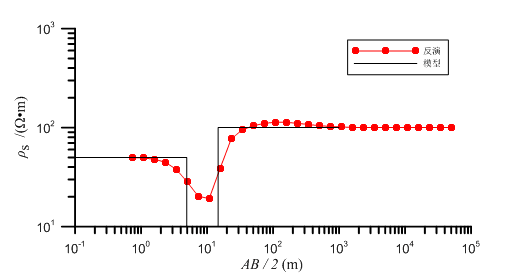
\includegraphics[scale=0.5]{1.png}
\caption{模型一}
\end{figure}
\begin{figure}[ht]
\centering
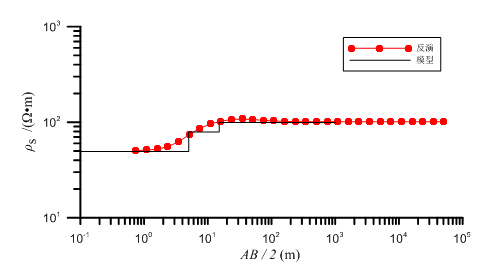
\includegraphics[scale=0.5]{2.png}
\caption{模型二}
\end{figure}
\begin{figure}[ht]
\centering
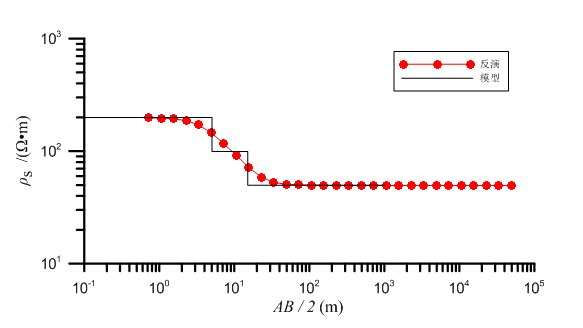
\includegraphics[scale=0.5]{3.png}
\caption{模型三}
\end{figure}
\begin{figure}[ht]
\centering
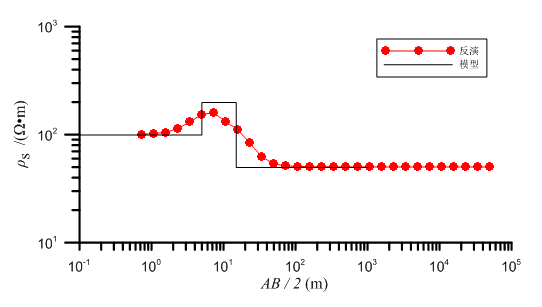
\includegraphics[scale=0.5]{4.png}
\caption{模型四}
\end{figure}

对比可发现,反演所得到的模型误差在可接受范围内,效果很好。
\end{document}
